%!TEX program = xelatex

% Name           : coq-hsrm-beamer-minimal.tex
% Author         : Tanja Almeroth (tanja.almeroth@mailbox.org)

% Copyright      : Copyright (c) 2020 by Tanja Almeroth. All rights reserved.
% License        : This file may be distributed and/or modified under the
%                  GNU Public License.
% Build up on the: HSRM beamer theme minimal example.
%                  (https://github.com/benjamin-weiss/hsrmbeamertheme)

% syntaxhighlighting for Gallina (Coq) listings
% see (https://github.com/nickgian/thesis)

\documentclass{beamer}
\graphicspath{{pics/}} % searchpath for graphics
\usepackage[english]{babel}
\usepackage{multicol}
%Erweiterte Tabellenfunktionen
\usepackage{tabularx,ragged2e}
\usepackage{booktabs}
% Listingserweiterung




\usepackage{listings}
\usepackage{lstcoq}
\lstset{language=coq, % Coq
		tabsize=4, % Tabulatorbreite
		linewidth=\linewidth, % Width of a line
		breaklines=true, % Break long lines
		breakatwhitespace=true, % Only break at whitespaces
		basicstyle=\scriptsize\ttfamily, % Schriftart/-größe
		numbers=left, % Linenumbers left
		numberfirstline=false, % Not: Always number 1. line
		numberstyle=\scriptsize, % Größe der Zeilennummern
		stepnumber=1, % Jede 2. Zeilennummer anzeigen
		numbersep=5pt, % Abstand Nr - Quellcode
		showspaces=false, % Spaces nicht anzeigen
		showtabs=false, % Tabs nicht anzeigen
		showstringspaces=false, % Don't show tabs in strings
		showlines=false, % Leerzeilen am Sourceende weglassen
		extendedchars=true, % ASCII-Zeichnen > 127 zulassen
		identifierstyle=\bfseries, % Identifier
		keywordstyle=\bfseries, % Keywords
		commentstyle=\itshape, % Style of comments
		stringstyle=\ttfamily, % Strings (!= Keywords)
		flexiblecolumns=false, % Use fixed width for fonts
		fontadjust=true, % "Base width" nicht jede Zeile anpassen
		frame=trbl, % Frame; trBL
		captionpos=b, % Position of the caption
		aboveskip=25pt}% Space between text and the top of the listing
		
%----------------------------------------------------------------------
% Load theme
\usetheme{hsrm}
%----------------------------------------------------------------------

% see slide logic using tikzpicture
%\usepackage{dtklogos} % must be loaded after theme
%\usepackage{tikz}
%\usetikzlibrary{mindmap,backgrounds}

%claim environment
\newenvironment{claim}[1]{\par\noindent\underline{Claim:}\space#1}{}
\newenvironment{claimproof}[1]{\par\noindent\underline{Proof:}\space#1}{\hfill $\blacksquare$}

%-----------------------------------------------------------------------
% title page
\title{A Brief Introduction To Coq}
\subtitle{The Coq Proof Assistant and Schedulability Analysis}
\author{Tanja Almeroth}
\institute{Studienbereich DCSM\\Hochschule {\Medium RheinMain}}
\date{\today}


\begin{document}
	
	\maketitle
		
% table of contents
	\section*{table of contents}
	
		\begin{frame}
			\frametitle{table of contents}
			\tableofcontents[hideallsubsections]
		\end{frame}
	
	
% start of presentation 

%%%%%%%%%%%%%%%%%%%%%%%%%%%%%%%%%%%%%%
% section about RECAP
%%%%%%%%%%%%%%%%%%%%%%%%%%%%%%%%%%%%%%

	\section{Recap}
	
	\begin{frame}{last time}
		\begin{itemize}
			\item proof assistants
			\item functional programming in Coq
			\item applications of Coq
			\item PROSA	and RT-Proofs
		\end{itemize}
	\end{frame}


	\begin{frame}{former Outlook}
		 \begin{itemize}
		 	 \item lecture notes for Steffen Reith, incorporate  review
		 	 \item incorporate linear temporal logic
			  \item Steffen Reith's review 
			  \item incorporate Steffen Reith's review on the PROSA working directory
		      \item tutorial on \texttt{Gallina} and \texttt{SSreflect} (4 person days)
			   \item formally proof the Kaiser's EDF scheduler in PROSA hopefully less then ($\approx 1'320$ LOC)
			  \item see at what is the best way to approach the complete kernel
			  
			  \end{itemize}
	 \end{frame}
	 
	
	\section{formally prove Kaiser's EDF-Scheduler}
	
	
	\begin{frame}{PROSA formal SCHEDULABILITY ANALYSIS}	
		\begin{itemize}
			\item basic tools from logic
			\item precise claims about programs
			\item functional programming methods of programming and logical reasoning about programs
		 \end{itemize}
		  
		 \begin{figure}[h]
					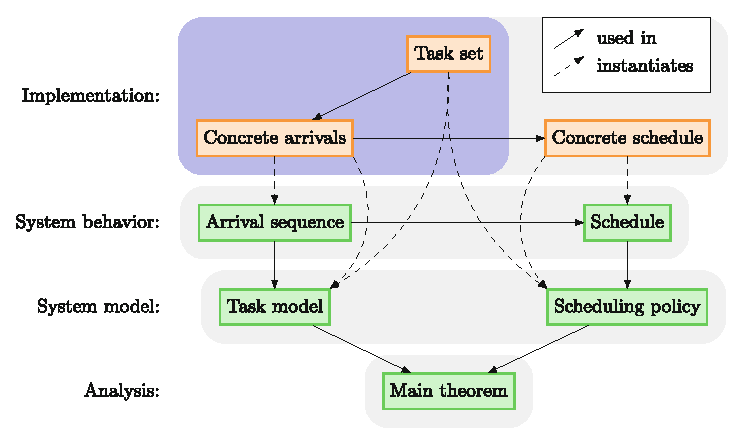
\includegraphics[width=.6\textwidth]{PROSALayers.eps}
					\label{fig:screenshot-proof-general}
					\caption{PROSA layers. Source:\cite{certikos_formal_schedulability}}
		 \end{figure}    	
		 
      \end{frame}
		  
		  
%	
%				  % 2 person years für RT Certikos- Real-Time extension
%              % Know-How about Certikos verification schon da gewesen in der Gruppe
%	           
	\begin{frame}{Main theorem: PROSA ECRTS16 Artifact Evalutaion}
     
	 practical specification: correctness of the proof 
	 		   
		 \begin{itemize}
	 	\item EDF-specific interference bound definition and proof of termination and correctness  of Bertongna and Cicerei's RTA for FP scheduling
		\item \alert{definition} \alert{and} \alert{proof} \alert{of} \alert{termination} \alert{and} \alert{correctness} \alert{of} \alert{Bertongna} \alert{and} \alert{Cicerei's} \alert{RTA} \alert{for} \alert{EDF} \alert{scheduling} \\($\approx 1'320$ LOC)    	   
		\end{itemize} 
			
	
    
    \begin{table}[]
			\begin{tabularx}{\linewidth}{l>{\raggedright}X}	
			my current working directory:\tabularnewline
			\url{https://gitlab.cs.hs-rm.de/almeroth/prosa_working_dir}\tabularnewline
			due to documentation including all listings
			($\approx 13'070$ \texttt{LOC})		
			\end{tabularx}
			\label{tab:Prosa_working_Dir}
			 
		\end{table}			 	
	
 	\end{frame}
			
	\section{LTL and multiprocessor scheduling}
	
	\begin{frame}{LTL and multiprocessor scheduling}
		Taxonomy of Multiprocessor Scheduling
		\begin{itemize}
			\item fixed task priority
			\item fixed job priority
			\item dynamic priority	
		\end{itemize}
	
	Idea: apply linear temporal logic to verify static and dynamic priority scheduling methods.\\
	Suggestion: Predicate logic-based approaches fail for dynamic priority scheduling methods. 	
	\end{frame}
	
		\begin{frame}{What is LTL}
		\begin{itemize}

			\item Linear temporal logic is linear like a linear tree (graph)
			 \item apply this linearity approach to a discrete time in a state-space system 
			\item LTL's origins are in the natural language descriptions
			\item natural numbers $\mathbb{N}$ represent a moment in time
					
		\end{itemize}
		Example: typical temporal operators
		\begin{itemize}
			\item $\bigcirc \phi$ means $\phi$ is true in the next moment 
			\item $\square \phi$  means $\phi$ is true in all future moments
			\item $\lozenge \phi$ means $\phi$ is true in some feature moment
			\item $\phi \mathcal{U} \psi$ means $\phi$ is true until $\psi$ is true
		\end{itemize}
			
			Goal: verification of dynamic priority scheduling methods  
	
	 	
	\end{frame}
	

		
%%%%%%%%%%%%%%%%%%%%%%%%%%%%%%%%%%%%%%%%%%%%	
% section programming in Coq	
%%%%%%%%%%%%%%%%%%%%%%%%%%%%%%%%%%%%%%%%%%%%
	

	% an example computation in Gallina	
%	\defverbatim[colored]	\CoqCompute{
%	\begin{lstlisting}[frame=single, emph={cout}, emphstyle=coq, label = lst:compute, caption = call \lstinline!Compute! ]
%	Compute (next_weekday friday).
%	\end{lstlisting}
%	\begin{lstlisting}[frame=single, emph={cout}, emphstyle=coq, label = lst:output, caption = output ]
%	= monday: day 
%	\end{lstlisting} 
%	}
	

%
%	\begin{frame}{an example}
%	\CoqCompute % example calculation
%	\end{frame}	
	% We computed something. E.g. called our first data type and function by name.
	% This is dynamic type reference in Coq. 
	% An 'std::cout>>"Hallo World";' in Coq.  


%%%%%%%%%%%%%%%%%%%%%%%%%%%%%%%%%%%%%%%%%%%%%%%%%%%%
% Applications
%%%%%%%%%%%%%%%%%%%%%%%%%%%%%%%%%%%%%%%%%%%%%%%%%%%%

	
	\section{Mutiprocessor scheduling}
	
	\begin{frame}{Problem}	
	In \emph{hard real-time systems}  we say a process or task is defined as an sequential execution of a program or a job on a processor.
	The execution ends after a \emph{finite number of steps}.

	$\rightarrow$\doublequoted{One big train of commands has to pass in a finite amount of time.}
	
	\begin{definition}
			\label{remark:problems}
			Multiprocessor scheduling can be viewed as attempting  to solve two problems.
			\begin{enumerate}[(i)]
				\item The \emph{allocation problem}, or on which processor the task should execute.
				\item The \emph{priority problem}, or in what order with respect to jobs of tasks each job should be executed.
			\end{enumerate}
		\end{definition}
	\end{frame}
	
  %%%%%%%%%%%%%
  %Let's call this the allocation and the priority problem
  % I read this paper with this error bounds
%%%%%%%%%%%%%%%%%%%%%%%%%%%%%%%%%%%%%%%%%%%%%%%%%%%%%%%%
% PROSA
%%%%%%%%%%%%%%%%%%%%%%%%%%%%%%%%%%%%%%%%%%%%%%%%%%%%%%%%	
 
      


%      
%      
%	\defverbatim[colored]\PROSAmaintheorem{%		
%		\begin{lstlisting}[emphstyle=coq, label = lst:theorem_edf_analysis, caption = \lstinline!theorem_edf_analysis! \cite{PROSA_ECRTS16ArtifcatEvaluation}]
%			Theorem edf_analysis_yields_response_time_bounds :
%        		∀ tsk R,
%          		(tsk, R) \\In edf_claimed_bounds ts →
%          		response_time_bounded_by tsk R. 
%		\end{lstlisting}
%      }       

	
%%%%%%%%%%%%%%%%%%%%%%%%%%%%%%%%%%%%%%%%%%%%%%%%%%%%%%%%%%%%%%	
% PROSA - formally proven schedubility analysis: Let's Play! 
%%%%%%%%%%%%%%%%%%%%%%%%%%%%%%%%%%%%%%%%%%%%%%%%%%%%%%%%%%%%%%

 	
 	\begin{frame}{Priority Problem}
		Kasier's  encapsulated EDF-scheduler \cite{K}
		\begin{itemize}
			\item real-time as in \cite{KBK}
			\item hierarchical (local and global distinction)
			\item multi-core (in the real-time-sense)
			\item EDF (earlines deadline first on a local level)
			\item sporadic 
			\item disruptive
		\end{itemize}	
		Main theorem: correctness of analysis although it is a deductive derivation				
 	\end{frame}

%%%%%%%%%%%%%%%%%%%%%%%%%%%%%%%%%%%%%%%%%%%%%%%%%%%%%%%%%%%%%%%%%%%%%%%%%%%%%%%
% In the following just copy conetnt from the lecture note file "TheKasiersSchedule.tex"
% If it is to boring, use an import from the repro.
%%%%%%%%%%%%%%%%%%%%%%%%%%%%%%%%%%%%%%%%%%%%%%%%%%%%%%%%%%%%%%%%%%%%%%%%%%%

%%%%%%%%%%%%%%%%%%%%%%%%%%%%%%%%%%%%%%%%%%%%%%%%%%%%%%%%%%%%%%%%%%%%%%%%%%%
% Definition of a job
%%%%%%%%%%%%%%%%%%%%%%%%%%%%%%%%%%%%%%%%%%%%%%%%%%%%%%%%%%%%%%%%%%%%%%%%%%% 	
 	
 	\begin{frame}{problem: Define a job or  task}
 	\begin{definition}
Let      
\begin{align*} & \delta_p \in \mathbb{N} \quad \text{be a periodic disruptive process and}\\
 	&\delta_s \in  \mathbb{N} \quad \text{be an asporadic disruptive process.}\\
	 &\text{Let} \quad P := \{1, \cdots, n \} \subset \mathbb{N}^n \\
	 &\quad \text{be a job, a set of disruptable processes}\\
	 &\quad \text{ with fixed priority order ascading.} \\
 	&\text{Let} \quad  \delta p_i \in \mathbb{N}, \quad \text{for} \quad i = 1,..,n \quad  \text{denote the period and}  \\
 	&\delta e_i \in \mathbb{N} \quad \text{for} \quad  i = 1,..,n \quad  \text{denote the execution time of a proces}.  
\end{align*}   
\end{definition}
 	\end{frame}
 	

	
	\begin{frame}{Multiprocessor scheduling algorithm}	
	\begin{definition}
We say a multiprocessor scheduling algorithm $\sigma$ is given by 
	\begin{align} 
	\sigma: &\mathbb{N}^n \times \mathbb{N}^n \longrightarrow  \mathbb{N} \times \{1,2,\cdots, m\} \\
	&\forall i, \delta e_j \in  \mathbb{N} \quad (i ,\delta e_j)  \mapsto (t,k) \in \mathbb{N}\times \{1,2,\cdots,m\}. 
	\end{align}
\end{definition}
  map time $i$ and execution time $\delta e_i$ to time-sequence $t$ and processor $k$ 		
 	\end{frame}
 	
 	
 	\begin{frame}{Multiprocessor scheduling algorithm}
 	
\begin{definition} A scheduler satisfying the EDF-regulation 
	\begin{equation}
	U(P) = \sum\limits_{i=1}^n \frac{\delta e_i}{\delta p_i} \leq 		\frac{\Delta e_{sv}}{\Delta p_{sv}}
	\end{equation}
	is called feasible.
\end{definition}	


 	\begin{theorem}
		A hard-real-time, hierarchical, multi-core, EDF, sporadic and disruptive time scheduler is feasible iff 
			\begin{align}
	\sum_{i=1}^n \lfloor \frac{t}{\Delta p_i} \rfloor \Delta e_i \leq \lfloor  \frac{t}{\Delta p_{sv}} \rfloor \Delta e_{sv} + \max (0,t  mod \Delta p_{sv} -\Delta e_{s} -\Delta e_p).
			\end{align}
		\end{theorem}
	\end{frame}
 	
 	

 	

%%%%%%%%%%%%%%%%%%%%%%%%%%%%%%%%%%%%%%%%%%%%%%%%%%%%%%%%
%	outlook 
%%%%%%%%%%%%%%%%%%%%%%%%%%%%%%%%%%%%%%%%%%%%%%%%%%%%%%%%	

	\begin{frame}{Outlook}
	apply the theorem of Akra -Bazzi
    	
	\end{frame}

	
	
	% Let's talk about verifiying an OS
	% Maroon
	% was kann das
	% wie groß ist das
	% ihr baut andauernd daran rum?
	% das Betreibssystem aus dem Airbus?
	
   % Linux Realtime Patch?   MPI-SWS hat einen.	
	
	
	% let's talk about Ada- and Maroon
	% LOC Ada code
	% LOC Marron Scheduler
	
	% Kaiser's Scheduler? 
	% I don't know
	% Wurde der nicht verkauf?
	% Können wir den noch benutzen?
	
	
	
	
%%%%%%%%%%%%%%%%%%%%%%%%%%%%%%%%%%%%%%%%%%%%%%%%%%%%%%%%%%%%%%%%%%%%%%%%%%%%%%%%%%%%%% 
% Books 
%%%%%%%%%%%%%%%%%%%%%%%%%%%%%%%%%%%%%%%%%%%%%%%%%%%%%%%%%%%%%%%%%%%%%%%%%%%%%%%%%%%%%%%	
	
	\begin{frame}{Bibliography}
		\begin{thebibliography}{10}
		\beamertemplatebookbibitems
		
		
		\bibitem{PACGGHSY2019}
		B. C.~ Pierce and A. A.~de Amorim and C.~Casinghino and M.~Gaboardi and M.~Greenberg and C.~Hriţcu and V.~Sjöberg and B.~Yorgey
		\newblock \doublequoted{Software Foundations, Logical foundations, Volume 1}
		\newblock \url{https://softwarefoundations.cis.upenn.edu/current/lf-current/index.html}, 2019
			
		\bibitem{COQ}
		Coq- Project Website	
		\newblock \doublequoted{The Coq Proof Assistant}
		\newblock \url{https://coq.inria.fr} , 2019-01-09
		
		
		\bibitem{RTproofs}
		RT-Proofs Website
		\newblock \doublequoted{Formal Proofs for Real-Time Systems}	
		\newblock \url{https://rt-proofs.inria.fr}, 2020-14-02		
		\end{thebibliography}	
	\end{frame}	
	
%%%%%%%%%%%%%%%%%%%%%
% IDES bibliography
%%%%%%%%%%%%%%%%%%%%%	

	\begin{frame}{Bibliography}{Coq}
		\begin{thebibliography}{10}
		\beamertemplatebookbibitems
		
		\bibitem{coqide}
		Coq Integrated Development Environment - Offical Documentation
		\newblock \doublequoted{Coq Integrated Development Environment}
		\newblock \url{https://coq.inria.fr/refman/practical-tools/coqide.html}		
				
		\bibitem{PG}
		Proof General - Project Website
		\newblock \doublequoted{Proof General, a generic interface for proof assitants.}
		\newblock \url{https://proofgeneral.github.io/}, 2020-14-02
		
		\bibitem{coquille}
		Coquille - Andreas Werner's Fork
		\newblock \doublequoted{Coquille, a vim plugin.}
		\newblock \url{https://github.com/Werner2005/coquille}, 2020-14-02		
		\end{thebibliography}
	\end{frame}
	
	
%%%%%%%%%%%%%%%%%%%%%%
% Coq online  	
%%%%%%%%%%%%%%%%%%%%%%

\begin{frame}{Bibliography: Online}
	\begin{thebibliography}{10}
		\beamertemplatebookbibitems
		
		\bibitem{syntaxhighliting}		
		N. Giannarakis
		\newblock Coq - Syntax Highlithing
		\newblock \doublequoted{Personal GitHub Profile}
		\newblock \url{https://github.com/nickgian/thesis/lstcoq.sty}, 2019-19-09		

	
		
		\end{thebibliography}
	
\end{frame}		
	
%%%%%%%%%%%%%%%%%%%%%%%%%%%%%%%%%
% Real-Time Systems
%%%%%%%%%%%%%%%%%%%%%%%%%%%%%%%%%%


	\begin{frame}{Bibliography: Real-Time Systems}
		\begin{thebibliography}{10}
			\beamertemplatebookbibitems
			
		
			\bibitem{KBK}		
			R. Kaiser and K. Beckmann and R. Kröger
			\newblock \doublequoted{Echtzeitplanung}
			\newblock Handouts \url{https://www.cs.hs-rm.de/~kaiser/1919_ezv/6_Scheduling-handout.pdf} 2020-07-01
			
			\bibitem{L}
			J. W.S. Liu
			\newblock \doublequoted{Real-time Systems}
			\newblock Prentice-Hall, Inc., ISBN: 0-13-099651-3, 2000
			
			\bibitem{K}
			R. Kasier 
			\newblock \doublequoted{Virtualisierung von Mehrprozessorsystemen mit Echtzeitanwendungen}
			\newblock PHD Thesis, Universität Koblenz-Landau, 11-02-2009
		\end{thebibliography}
	
	\end{frame}		
	

\begin{frame}{Bibliography: Real-Time Systems}
	\begin{thebibliography}{10}
		\beamertemplatebookbibitems		
		
		\bibitem{B}
		G. Bollella 
		\newblock \doublequoted{Slotted Priorities: Supporting Real-Time Computing Within General-Purpose Operating Systems}
		\newblock PHD Thesis, Chapel Hill, 1997	
	
	    
	   	\beamertemplatearticlebibitems
	    
	    \bibitem{C}
	    M. Bertogna and M. Cirinei
	    \newblock \doublequoted{Response-Time Analysis for Globally Scheduled Symmetric Multiprocessor Platforms}
	    \newblock Proceedings of the 28th IEEE International Real-Time Systems Symposium (RTSS 07)
	    
			\end{thebibliography}
	    
  


\end{frame}		



%%%%%%
% Conference Papers
%%%%%%
		
	
%@InProceedings{10.1007/978-3-030-25543-5_28,
%	author="Guo, Xiaojie and Lesourd, Maxime and Liu, Mengqi and Rieg, Lionel and Shao, Zhong",
%	editor="Dillig, Isil
	%and Tasiran, Serdar",
	%title="Integrating Formal Schedulability Analysis into a Verified OS Kernel",
	%booktitle="Computer Aided Verification",
	%year="2019",
	%publisher="Springer International Publishing",
	%address="Cham",
	%pages="496--514",
	%abstract="Formal verification of real-time systems is attractive because these systems often perform critical operations. Unlike non real-time systems, latency and response time guarantees are of critical importance in this setting, as much as functional correctness. Nevertheless, formal verification of real-time OSes usually stops the scheduling analysis at the policy level: they only prove that the scheduler (or its abstract model) satisfies some scheduling policy. In this paper, we go further and connect together Prosa, a verified schedulability analyzer, and RT-CertiKOS, a verified single-core sequential real-time OS kernel. Thus, we get a more general and extensible schedulability analysis proof for RT-CertiKOS, as well a concrete implementation validating Prosa models. It also showcases that it is realistic to connect two completely independent formal developments in a proof assistant.",
	%isbn="978-3-030-25543-5"
	%}		
	%
	%
	%
	%
	%
	%
	%

%%%%%%%%%%%%%%%%%%%%%%%%%%%%%%%%%%%%%%%%%%%%%%%%%%%%%%%%
% Operating Systems Literature
%%%%%%%%%%%%%%%%%%%%%%%%%%%%%%%%%%%%%%%%%%%%%%%%%%%%%%%%
		
	\begin{frame}{Bibliography: Real-Time Systems}
		\begin{thebibliography}{10}
		\beamertemplatebookbibitems
		
		\bibitem{PROSA_ECRTS16ArtifcatEvaluation}
		F.~ Cerqueira and  F. ~ Stutz, and B.~ Brandenburg
		\newblock \doublequoted{Prosa - ECRTS’16 Artifact Evaluation}
		\newblock \url{https://prosa.mpi-sws.org/releases/v0.1/artifact/},  2020-01-09
		
		\beamertemplatearticlebibitems
		
		\bibitem{PROSA_schedubility_analysis }		
		F.~ Cerqueira and  F. ~ Stutz, and B.~ Brandenburg		
		\newblock \doublequoted{PROSA: A Case for Readable Mechanized Schedulability Analysis}	
		\newblock \url{https://www.mpi-sws.org/~bbb/papers/pdf/ecrts16f.pdf}
		\newblock Proceedings of the 28th Euromicro Conference on Real-Time Systems (ECRTS), 2016	
		\end{thebibliography}	
	\end{frame}		
	
%%%%%%%%%%%%%%%%%%%%%%%%%%%%%%%%%%%%%%%%%%%%%%%%%%%%%%%
% Compiler Stuff
%%%%%%%%%%%%%%%%%%%%%%%%%%%%%%%%%%%%%%%%%%%%%%%%%%%%%%%%
	
	\begin{frame}{Bibliography: Computer and Communication Security}
		\begin{thebibliography}{10}
			\beamertemplatearticlebibitems
		
			\bibitem{JASMIN}
		Almeida, Jos\'{e} Bacelar and Barbosa, Manuel and Barthe, Gilles and Blot, Arthur and Gr\'{e}goire, Benjamin and Laporte, Vincent and Oliveira, Tiago and Pacheco, Hugo and Schmidt, Benedikt and Strub, Pierre-Yves
			\newblock \doublequoted{Jasmin: High-Assurance and High-Speed Cryptography}
			\newblock Proceedings of the 2017 ACM SIGSAC Conference on Computer and Communications Security (CCS), 2017
		\end{thebibliography}
	 \end{frame}
	 
	
%%%%%%%%%%%%%%%%%%%%%%%%%%%%%%%%%%%%%%%%%%%%%%%%%%%%%%%
% Verifying an OS -Kernel
%%%%%%%%%%%%%%%%%%%%%%%%%%%%%%%%%%%%%%%%%%%%%%%%%%%%%%%%	 
	 
	 \begin{frame}{Bibliography: Verifying an OS Kernel}
	 	\begin{thebibliography}{10}
	     \beamertemplatebookbibitems	
	      	
	 	 \bibitem{certikos_formal_schedulability}
	 Guo, Xiaojie and Lesourd, Maxime and Liu, Mengqi and Rieg, Lionel and Shao, Zhong 
	 \newblock \doublequoted{Integrating Formal Schedulability Analysis into a Verified OS Kernel}
	 \newblock Computer Aided Verification, Springer International Publishing
	 \newblock 2019
		\end{thebibliography}
	\end{frame}

	 
	
	 
	% Examples from latex Template	
	%	\beamertemplatearticlebibitems
		
		
	%	\beamertemplatebookbibitems
	%	\bibitem{Oppenheim2009}
	%	Alan~V.~Oppenheim
	%	\newblock \doublequoted{Discrete-Time Signal Processing}
	%	\newblock Prentice Hall Press, 2009
	%
	%	\beamertemplatearticlebibitems
	%	\bibitem{EBU2011}
	%	European~Broadcasting~Union
	%	\newblock \doublequoted{Specification of the Broadcast Wave Format (BWF)}
	%	\newblock 2011
	


\end{document}






